\documentclass[../main.tex]{subfiles}
\begin{document}

\section{Experimental Setup}
The purpose of the experiment is the estimation of the lifetime of the muon, via the determination of the time elapsed between the passage of a muon and its decay. In order to perform this measurement, an appropriate experimental setup has been devised. For the full list of used instrumentation check Appendix \ref{appendix:instruments}.


\subsection{Scintillator Planes}
The experimental setup is composed of 3 scintillator planes (P1, P2, P3) with a surface of \mbox{$\approx$\SI{600}{\centi \metre^2}} and a thickness of $\approx$\SI{2.5}{\centi \metre}. 
Each plane is composed of 2 plastic scintillator planes joint in the middle and 2 Hamamatsu H316504 photomultipliers (PMTs). The PMTs are coupled to the scintillating planes, having them face one another at different ends of the planes. PMTs are powered by a NIM power supply unit, controlled by the CAEN GEneral COntrol (GECO) software. Both the PMTs on the same plane are powered by a single cable, therefore working at the same settings. The output signal of each PMT is carried to the rack via 50\,$\Omega$ LEMO coaxial cables, each of them introducing delays in the order of nanoseconds depending on the length of the used cable. The render of an experimental plane is shown in Figure \ref{fig:plane}.

\begin{figure}[htb]
    \centering
    \includegraphics[width=0.5 \linewidth]{images/plane.png} \hspace{0.3 cm}
    \includegraphics[width=0.3 \linewidth]{images/plane3.png}
    \caption{Schematics of the scintillating plane and PMT details.}
    \label{fig:plane}
\end{figure}

\subsection{Signal Processing and Data Acquisition}
All signals require later processing according to the proper purposes that have to be carried out, later discussed in the relevant sections. Since the output of the PMT is an analog signal the use of a CAEN N840 8-Channel Leading Edge Discriminator (LED) for the conversion into a digital signal will be assumed throughout all the following discussions.

Another important step in the signal processing requires the use of logic AND ($\land$) and OR ($\lor$) operations. In order to achieve this CAEN N455 Quad Coincidence Logic Unit and CAEN N405 3 Fold Logic Unit have been used, typically the first one for outputs of the PMTs, the second instead for logic operations on the outputs of the previous unit.

For generation of time signals the CAEN N93B Dual Timer unit has been used, in particular for the time calibration of the setup and for background measurement.

The CAEN N1145 Quad Scaler and Preset Counter Timer unit has been used to select the working points of the PMTs, and to perform efficiency and preliminary measurements. In particular, this unit allows to take 8-digits counts on up to 4 channels in specified and consistent time windows with up to \unit{\micro \second} resolution.

For trigger purposes and appropriate circuit response/data taking to compensate for different delays in different channels the CAEN N108A Dual Delay could provide up to \mbox{$\approx$64\,ns} of delay.

Figure \ref{fig:rack} shows the rack during data taking.\\

\begin{figure}[htb]
    \centering
    \includegraphics[width=0.7 \linewidth]{images/rack.jpg}
    \caption{Rack during data taking.}
    \label{fig:rack}
\end{figure}

After exiting from the rack, signals can be sent either to an RS PRO IDS1104B Digital Oscilloscope, which can provide information on height and width of signals on up to 4 channels, or to a Digilent Cmod Spartan-7 FPGA. The FPGA contains a code for data acquisition which saves data in text (\texttt{.txt}) files into the laboratory PC. The FPGA features 4 connectors to the setup, 1 for the trigger and 3 for the acquisition channels given by the 3 scintillator planes. The output files will feature 3 values for each triggered event, each value being a stopping time expressed in clock ticks units, one for each one of the planes. 

\subsection{Detector}
\label{sub:detector}
In order to observe a muon decay, some things have to be taken into account. 

Firstly,  muons may cross a plane from different directions. This experiment is mostly concerned with muons which have a vertical trajectory, coming from the Zenith. The configuration that enhances the probability of capturing such muons reducing spurious correlation of non vertical muons is the one in which two planes are put on top of one another. For data taking, a trigger has been constructed and the first action it performs is to check whether both planes signalled the passage of a muon.

Furthermore, since the interest lies in observing the decay of the muon it is important to remove events in which muons crossed the full detector without decaying. For this purpose the third plane, placed below the other two planes, acts as a veto on the aforementioned trigger.

Finally, when looking at the physics of the processes described in Section  \ref{sec:intro} cosmic muons are expected to be emitted in the $10^2-$\SI{e5}{\MeV} energy range, while for what concerns the processes described in (\ref{eq:muDecay}) the electron is expected to be emitted in the \SI{30}{MeV} energy range. In order to slow down the muon, it is necessary to add an absorber between planes so that the muon can lose enough energy to slow down and decay, while at the same time allowing the daughter electron to escape the decay region reaching the detection region. A fine compromise between the two things is using an absorber in which a \SI{30}{\MeV} electron has a high enough probability to escape. Taking into account also cost constraints, a \SI{1}{cm} iron absorber plate was used. Future modifications to the setup may also include the introduction of a magnetic field for the identification of the charge of passing particles. For this reason, also a \SI{4}{\centi \meter} concrete absorber has been tested since iron, being ferromagnetic, would be a problematic absorber inside a magnetic field.\\


\noindent For the previously discussed reasons the detector has been constructed as shown in Figure \ref{fig:setUp}.

\begin{figure}[htb]
    \centering
    \tikzset{every picture/.style={line width=0.75pt}} %set default line width to 0.75pt        

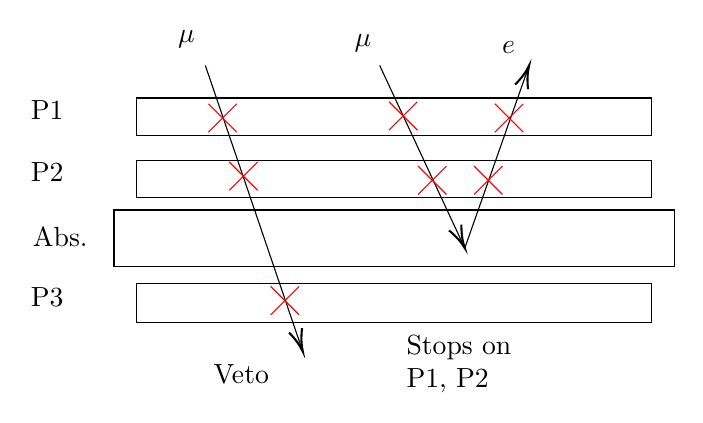
\begin{tikzpicture}[x=0.75pt,y=0.75pt,yscale=-1,xscale=1]
%uncomment if require: \path (0,239); %set diagram left start at 0, and has height of 239

%Shape: Rectangle [id:dp779608831693803] 
\draw   (131,81) -- (379.33,81) -- (379.33,99) -- (131,99) -- cycle ;
%Shape: Rectangle [id:dp6210994436881714] 
\draw   (131,170.33) -- (379.33,170.33) -- (379.33,189) -- (131,189) -- cycle ;
%Shape: Rectangle [id:dp18252585112175712] 
\draw   (120.33,135) -- (390.33,135) -- (390.33,162) -- (120.33,162) -- cycle ;
%Shape: Rectangle [id:dp9173904155089121] 
\draw   (131,111) -- (379.33,111) -- (379.33,129) -- (131,129) -- cycle ;
%Straight Lines [id:da7511843328220018] 
\draw    (164.33,65.33) -- (210.69,201.44) ;
\draw [shift={(211.33,203.33)}, rotate = 251.19] [color={rgb, 255:red, 0; green, 0; blue, 0 }  ][line width=0.75]    (10.93,-3.29) .. controls (6.95,-1.4) and (3.31,-0.3) .. (0,0) .. controls (3.31,0.3) and (6.95,1.4) .. (10.93,3.29)   ;
%Straight Lines [id:da650554014246816] 
\draw    (248.33,65.33) -- (288.49,151.52) ;
\draw [shift={(289.33,153.33)}, rotate = 245.02] [color={rgb, 255:red, 0; green, 0; blue, 0 }  ][line width=0.75]    (10.93,-3.29) .. controls (6.95,-1.4) and (3.31,-0.3) .. (0,0) .. controls (3.31,0.3) and (6.95,1.4) .. (10.93,3.29)   ;
%Straight Lines [id:da9118596186922334] 
\draw    (289.33,153.33) -- (319.67,67.22) ;
\draw [shift={(320.33,65.33)}, rotate = 109.41] [color={rgb, 255:red, 0; green, 0; blue, 0 }  ][line width=0.75]    (10.93,-3.29) .. controls (6.95,-1.4) and (3.31,-0.3) .. (0,0) .. controls (3.31,0.3) and (6.95,1.4) .. (10.93,3.29)   ;
\draw  [color={rgb, 255:red, 255; green, 0; blue, 0 }  ,draw opacity=1 ] (165.83,83.83) -- (179.5,97.5)(179.5,83.83) -- (165.83,97.5) ;
\draw  [color={rgb, 255:red, 255; green, 0; blue, 0 }  ,draw opacity=1 ] (175.83,111.83) -- (189.5,125.5)(189.5,111.83) -- (175.83,125.5) ;
\draw  [color={rgb, 255:red, 255; green, 0; blue, 0 }  ,draw opacity=1 ] (195.83,171.83) -- (209.5,185.5)(209.5,171.83) -- (195.83,185.5) ;
\draw  [color={rgb, 255:red, 255; green, 0; blue, 0 }  ,draw opacity=1 ] (252.83,82.83) -- (266.5,96.5)(266.5,82.83) -- (252.83,96.5) ;
\draw  [color={rgb, 255:red, 255; green, 0; blue, 0 }  ,draw opacity=1 ] (266.83,113.83) -- (280.5,127.5)(280.5,113.83) -- (266.83,127.5) ;
\draw  [color={rgb, 255:red, 255; green, 0; blue, 0 }  ,draw opacity=1 ] (303.83,83.83) -- (317.5,97.5)(317.5,83.83) -- (303.83,97.5) ;
\draw  [color={rgb, 255:red, 255; green, 0; blue, 0 }  ,draw opacity=1 ] (293.83,113.83) -- (307.5,127.5)(307.5,113.83) -- (293.83,127.5) ;

% Text Node
\draw (79,81) node [anchor=north west][inner sep=0.75pt]   [align=left] {P1};
% Text Node
\draw (79,111) node [anchor=north west][inner sep=0.75pt]   [align=left] {P2};
% Text Node
\draw (79,171) node [anchor=north west][inner sep=0.75pt]   [align=left] {P3};
% Text Node
\draw (80,142) node [anchor=north west][inner sep=0.75pt]   [align=left] {Abs.};
% Text Node
\draw (167,208) node [anchor=north west][inner sep=0.75pt]   [align=left] {Veto};
% Text Node
\draw (150,47.4) node [anchor=north west][inner sep=0.75pt]    {$\mu $};
% Text Node
\draw (235,49.4) node [anchor=north west][inner sep=0.75pt]    {$\mu $};
% Text Node
\draw (306,52.4) node [anchor=north west][inner sep=0.75pt]    {$e$};
% Text Node
\draw (260,194) node [anchor=north west][inner sep=0.75pt]   [align=left] {Stops on\\ P1, P2};


\end{tikzpicture}
    \includegraphics[width = 0.4 \linewidth]{images/setup.jpg}
    \caption{Detector schematics and mounted experiment with concrete absorber.}
    \label{fig:setUp}
\end{figure}


\end{document}

\clearpage